% NeuroCam manual - IR modifications for Logitech c920.
% Written by Christopher Thomas.
% Copyright (c) 2021 by Vanderbilt University. This work is released under
% the Creative Commons Attribution-ShareAlike 4.0 International License.

\chapter{IR Modifications for Logitech C920 Camera}
\label{c920}

The Logitech C920 webcam can be readily modified for near-infrared use. This
involves the following actions:
\begin{itemize}
\item Disassembling the camera.
\item Removing the optics assembly from the board.
\item Removing the infrared filter from the optics assembly.
\item Replacing the infrared filter with glass plates of appropriate
thickness.
\end{itemize}

Detailed documentation of these actions is described below.

\section{Confirm Camera Identity}

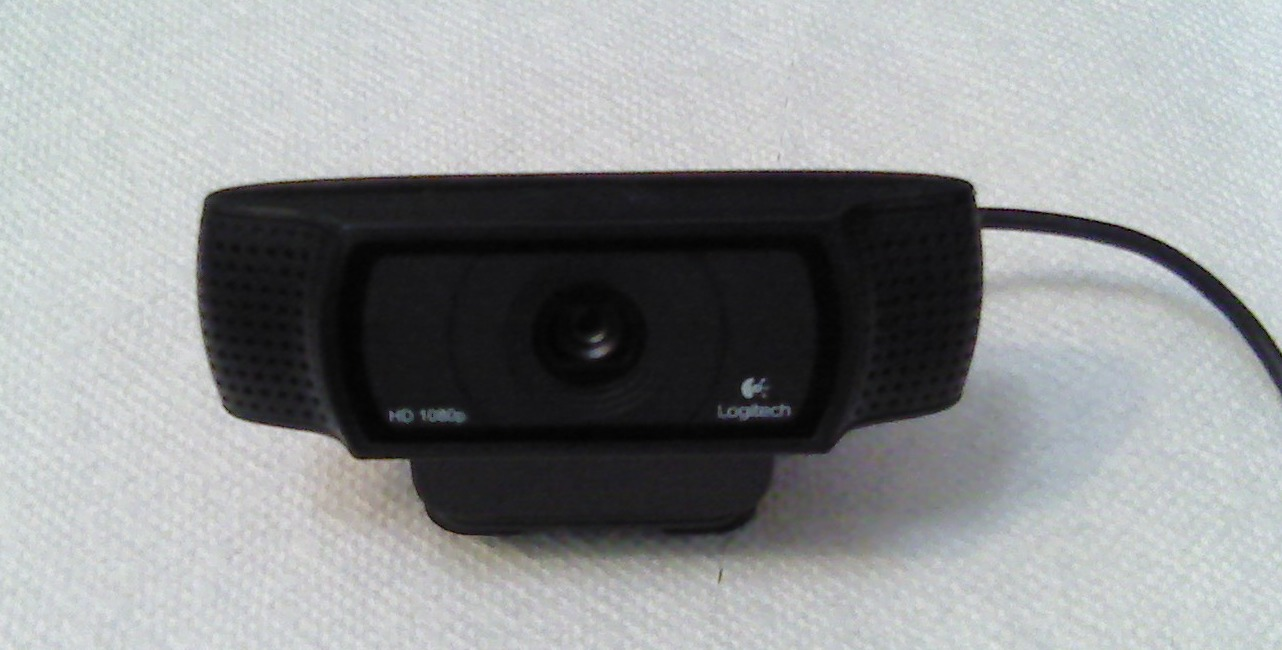
\includegraphics[height=2in]{pics-c920/01-start.jpg}

This documentation only applies to the Logitech C920 camera. Other cameras,
even closely-related models, have different internal layouts and methods of
disassembly.

\section{Remove Stickers and Microphone Guards}

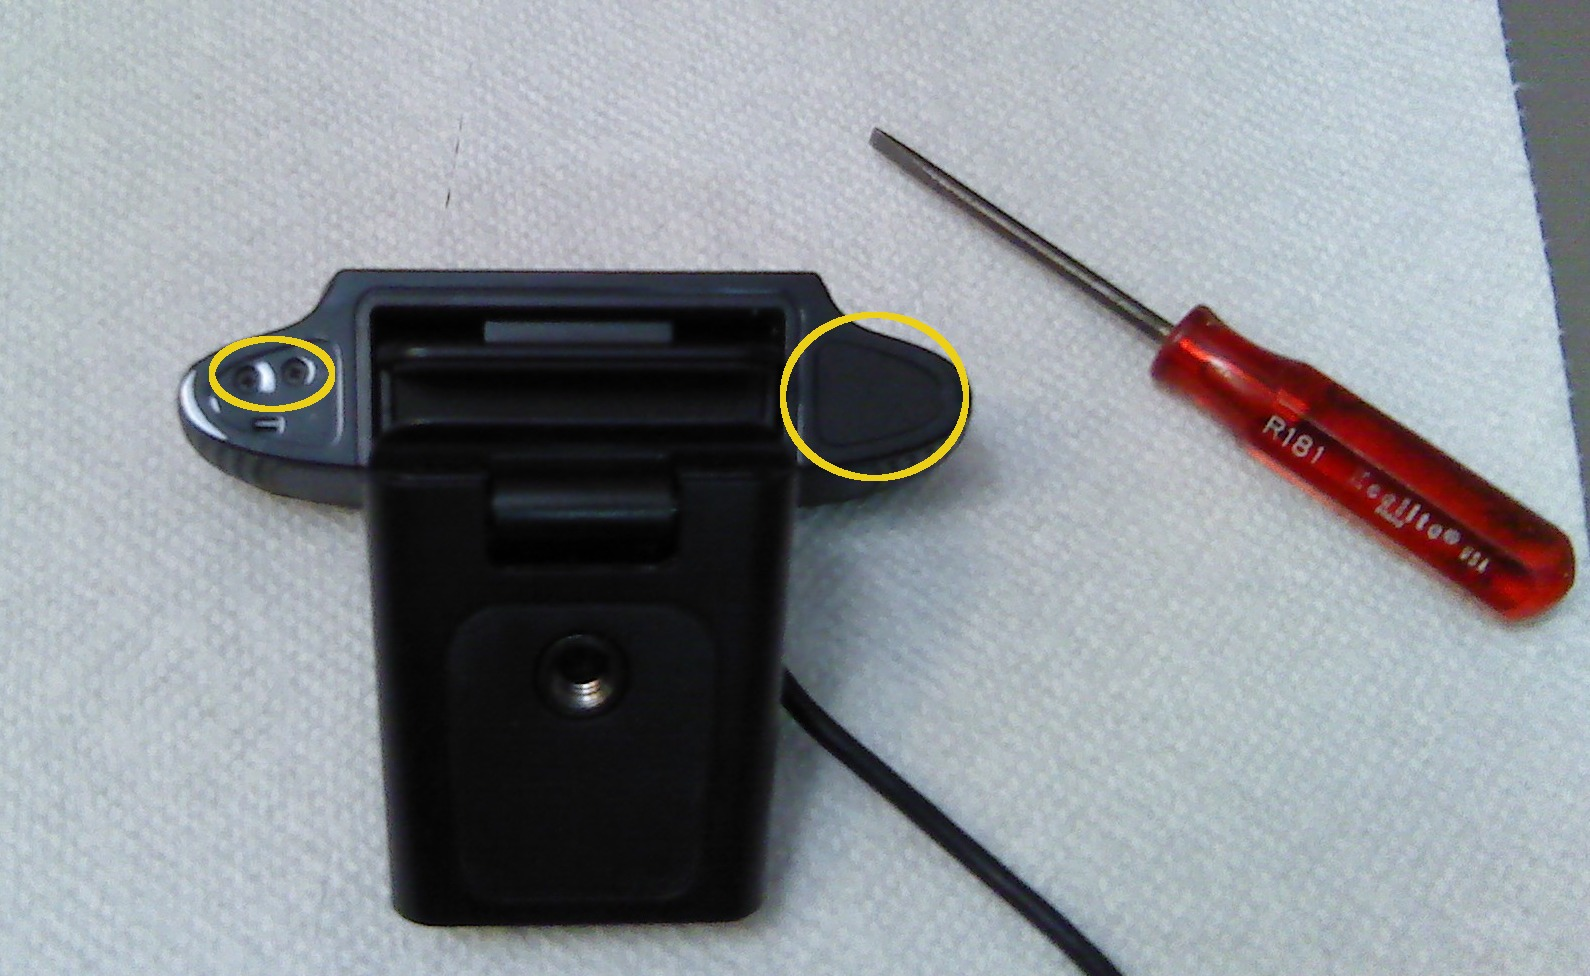
\includegraphics[height=2in]{pics-c920/02-bottomscrews.jpg}

The screws securing the microphone guards are covered by two layers of
stickers. Both layers must be removed to access them.

\section{Remove Cover}

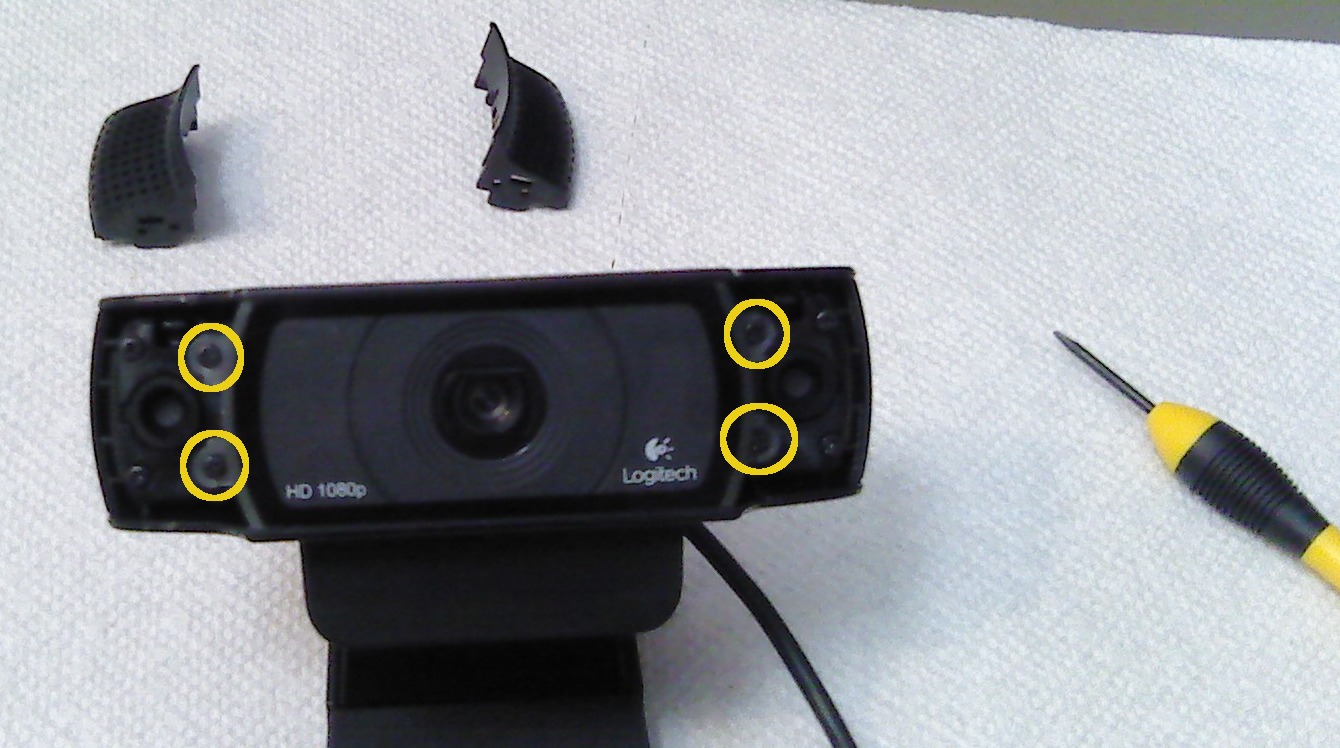
\includegraphics[height=2in]{pics-c920/03-coverscrews.jpg}

\section{Remove Mounting Bracket}

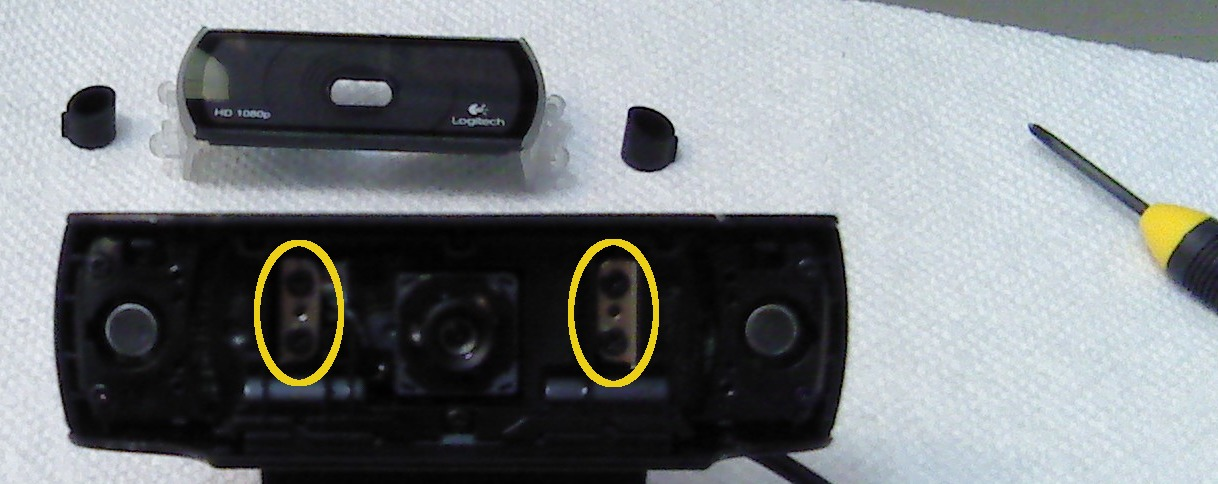
\includegraphics[height=2in]{pics-c920/04-bracketscrews.jpg}

There is a peg between each pair of bracket screws. To remove the mounting
bracket, rotate the bracket so that its metal flanges lift off of these pegs.
The flanges will then slide out of the camera easily.

\section{Remove Spacer}

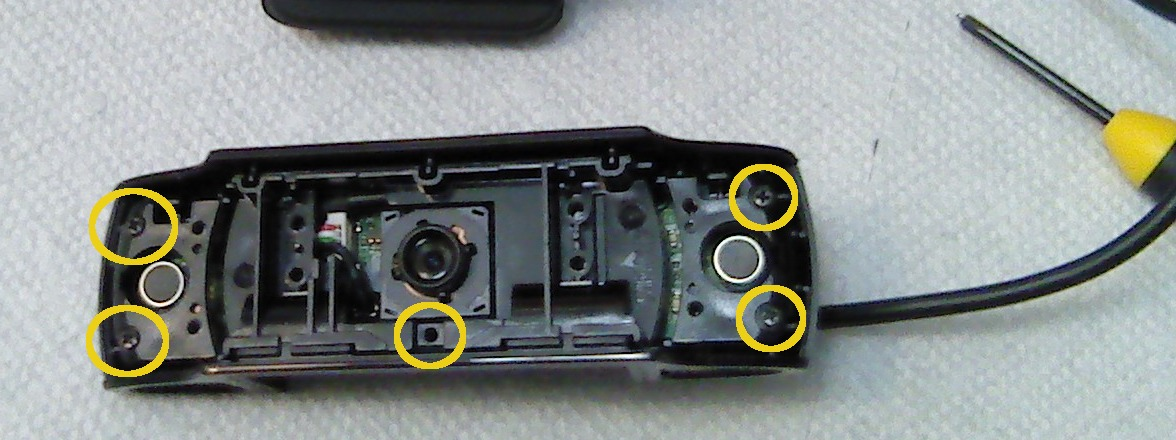
\includegraphics[height=2in]{pics-c920/05-spacerscrews.jpg}

\section{Remove Board}

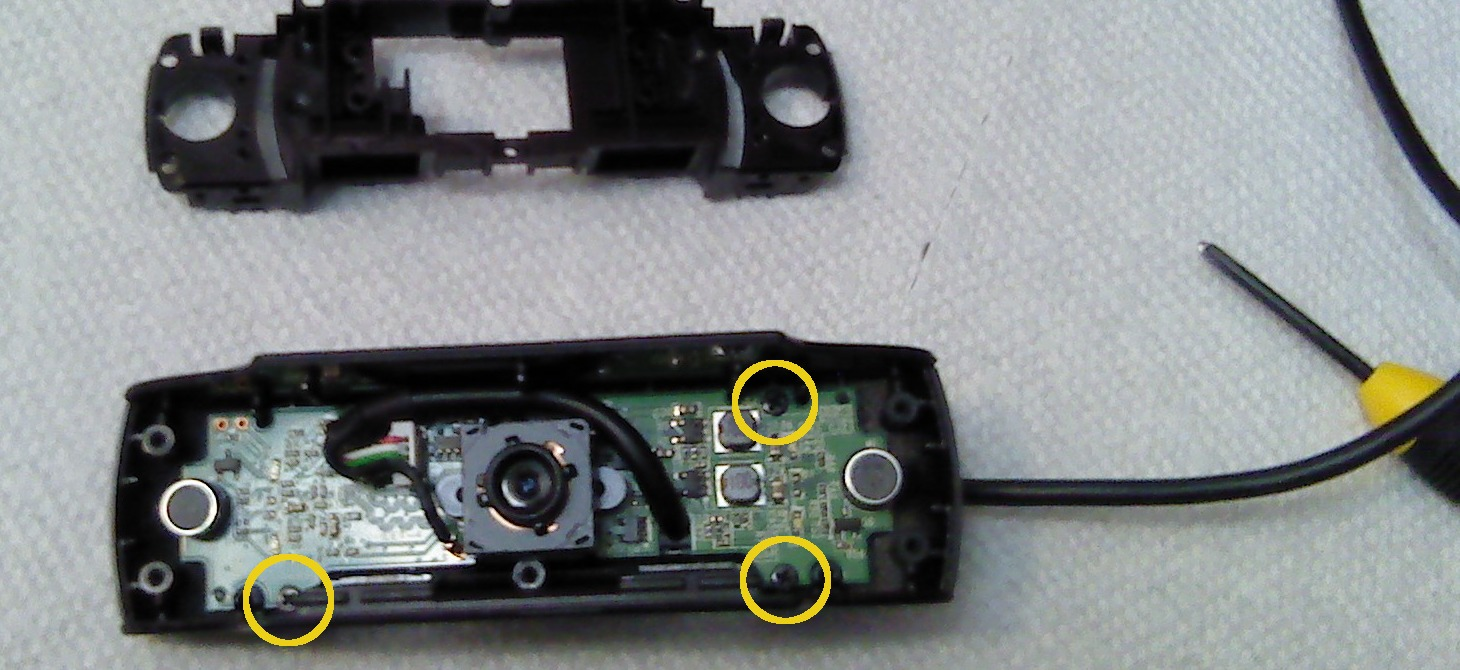
\includegraphics[height=2in]{pics-c920/06-boardscrews.jpg}

The USB cable is fixed to the case. The board can be removed by rotating it,
while bending the side of the case slightly to release the catches that secure
the board and the USB cable. Do not bend the board itself (that may destroy
it).

Alternatively, the USB cable can be unplugged from the board (via the header
and ground pin). This is risky, as both connectors are easy to damage.

\section{Optional: Remove LEDs}

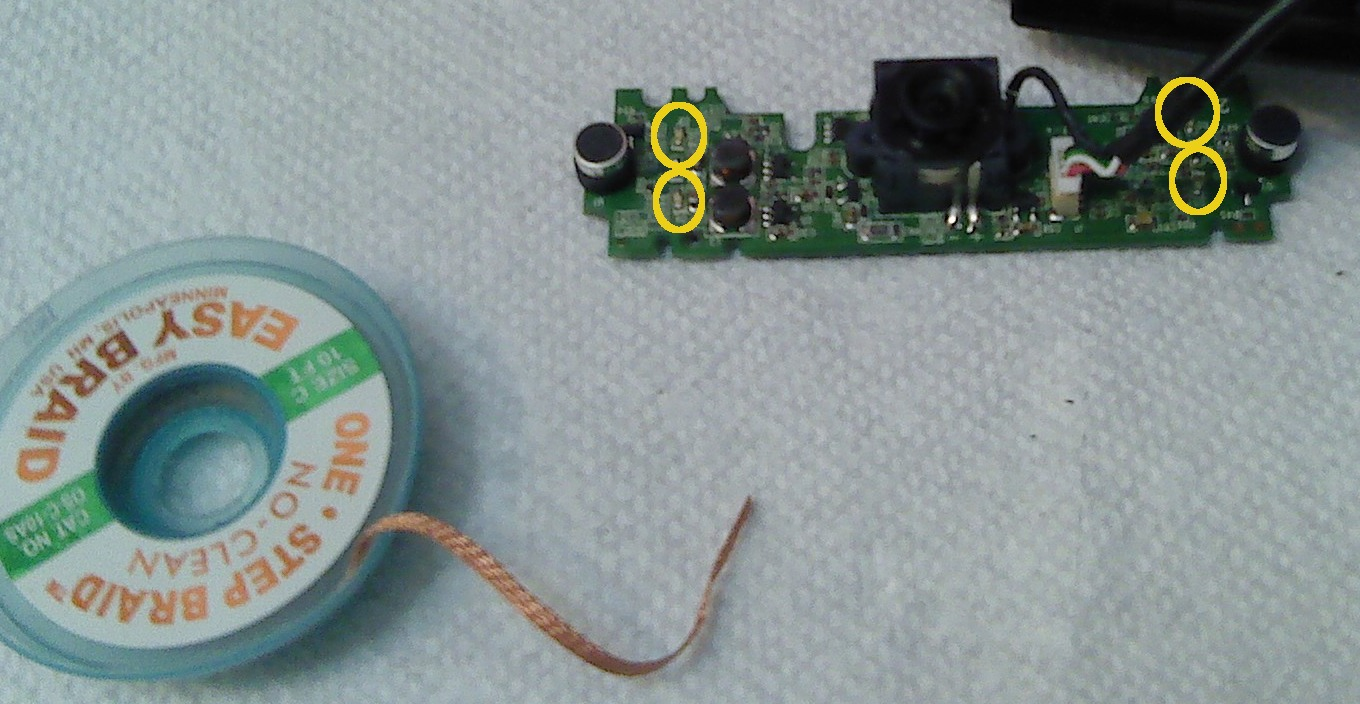
\includegraphics[height=2in]{pics-c920/06b-leds.jpg}

The camera status LEDs are white rectangular components with labels ``D3''
through ``D8''. Only four of the six positions are populated. These can be
removed using ``solder wick'' per Step \ref{sect-920-desolder} if desired.
Tearing pads is tolerable, as long as no other traces or components are
disturbed.

Do not use a heat gun. Hot air will desolder other nearby components and may
blow them out of position.

\section{Unscrew Optics Assembly}

\includegraphics[height=2in]{pics-c920/07-opticsscrews.jpg}

After being unscrewed, the optics assembly will remain secured to the board
by its soldered contacts.

\section{Un-Solder and Remove Optics Assembly}
\label{sect-920-desolder}

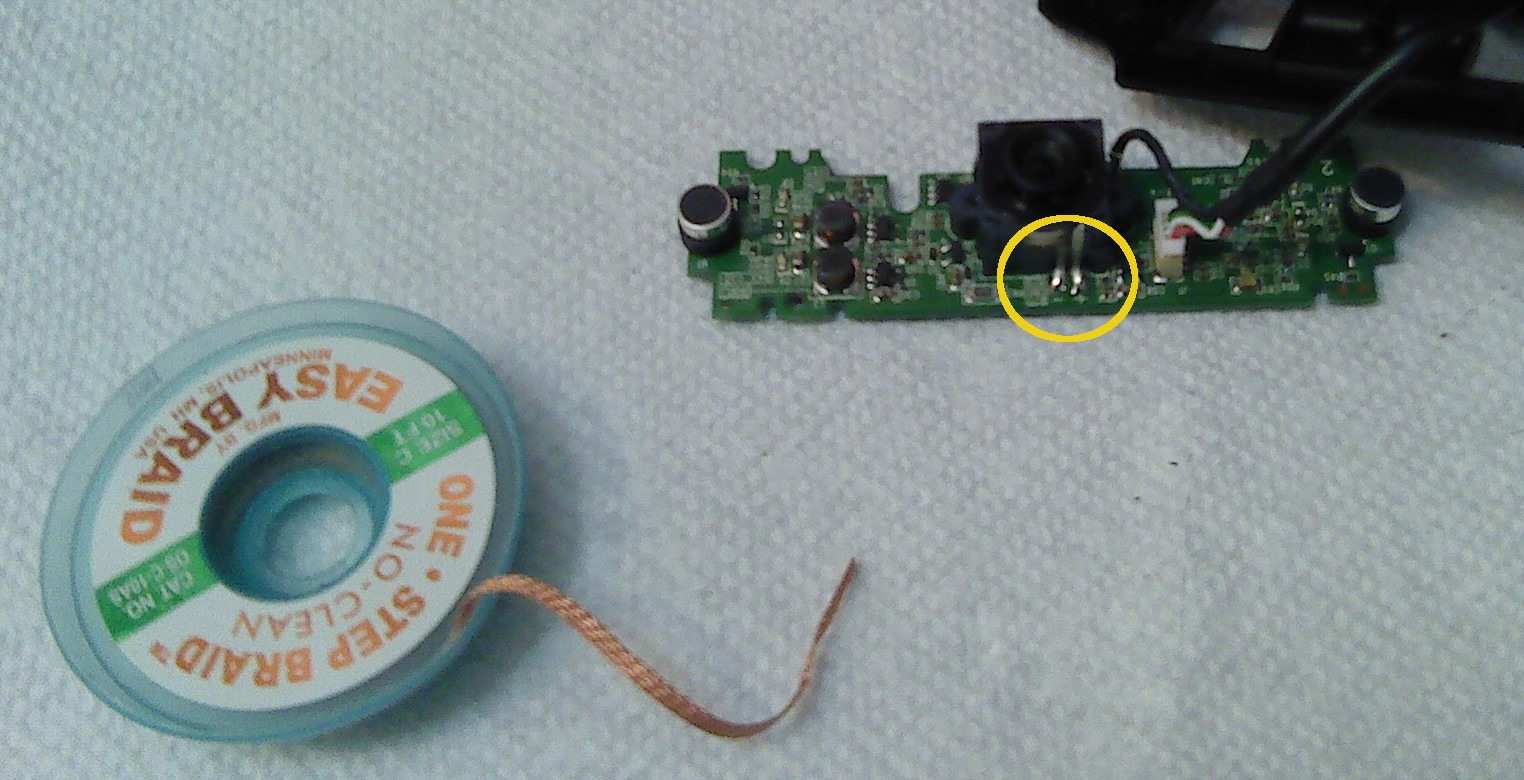
\includegraphics[height=2in]{pics-c920/08-opticsleads.jpg}

The optics assembly leads can be desoldered using ``solder wick'' (also
called ``desoldering braid''). A variety that has flux in the braid is
recommended (though flux can be applied separately if necessary). Setting
the iron to high temperature makes desoldering easier, but care must be
taken to avoid heat damage to nearby components.

Be gentle when removing the optics assembly, as the contact pads it's
soldered to can be torn off of the board if they're still partly bonded to
the leads.

Do not use a heat gun. The sensor die is nearby and may be damaged. The
anisotropic film holding the sensor die to the board may also be damaged.

\section{Verify Absence of Damage and Dust}

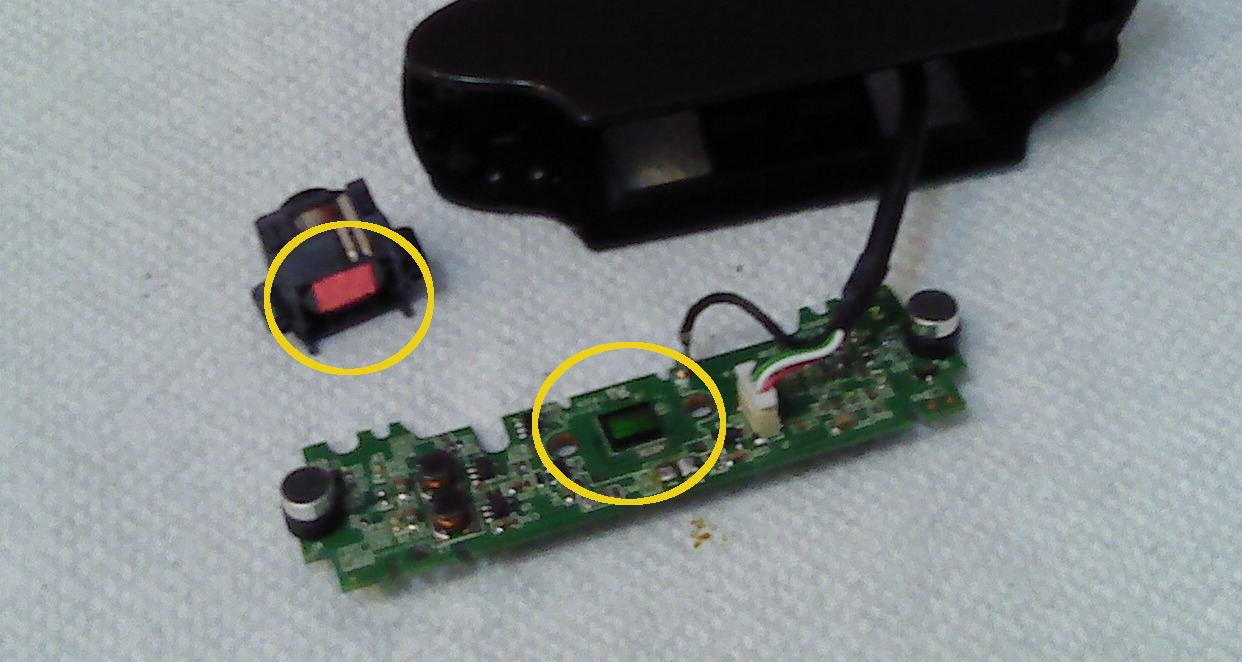
\includegraphics[height=2in]{pics-c920/09-filterdie.jpg}

The IR filter (in the optics assembly) and sensor die (on the board) are now
visible.

The sensor die is fragile (and has a fragile coating). It should be visually
inspected to confirm that no scratches or dust particles are present. Take
care not to breathe on it while inspecting it, as moisture will leave droplets
on the die.

If moisture or dust are present on the die, the die can be cleaned by wiping
it very gently using ``lens tissue'' (also called ``lens paper''). Wiping that
is not sufficiently gentle will instead scratch the die by dragging dust
particles across it.

The lens tissue may be soaked in alcohol prior to wiping. This makes it
easier to safely remove dust, and is the only way to remove water stains,
but it is possible that alcohol may damage the coatings on the die. Wipe
diagonally from one corner of the die to the other, to minimize the amount
of liquid that clings to the trailing edge of the die, and then wipe again
with a dry piece of lens tissue (or a dry corner of the same piece).

Do not allow alcohol to contact the anisotropic film holding the die to the
board, as it will likely cause delamination.

\section{Heat Infrared Filter}

\includegraphics[height=3in]{pics-c920/10-heatgun.jpg}

The infrared filter plate is bonded to the optics assembly with glue. Play a
heat gun around the edge of the filter plate to soften this glue. Use a
circular motion to avoid overheating any one part of the edge or allowing any
other part to cool. Use a low temperature setting to avoid cracking the plate
due to heat shock and to avoid melting the plastic housing.

\section{Remove Infrared Filter}

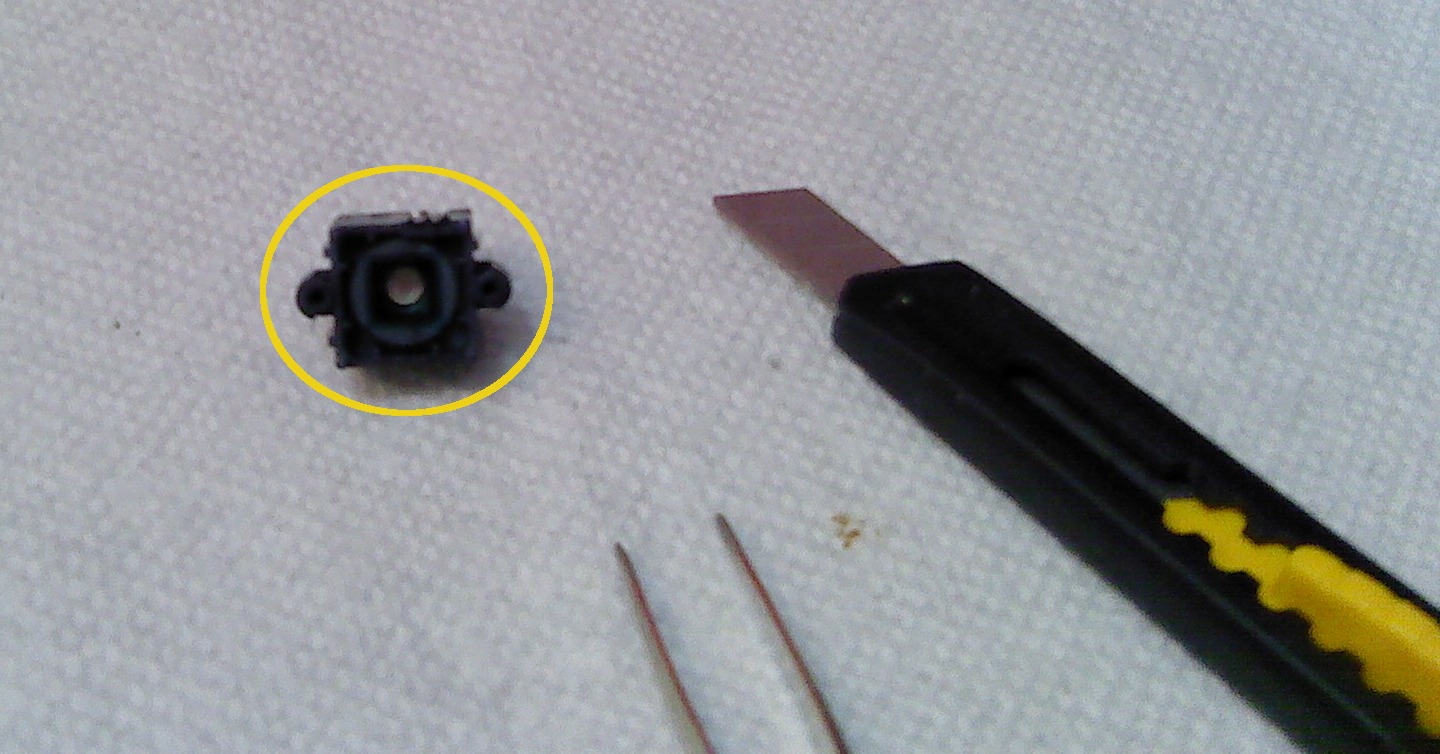
\includegraphics[height=2in]{pics-c920/11-knife.jpg}

Use the edge of a sharp knife to pry the filter plate out of the optics
assembly. Lift from one corner, letting the plate hinge on one of the
opposing edges. If there is any resistance, use the heat gun again to soften
the glue.

Discard the filter plate after removal.

\section{Scribe Microscope Cover Slips}

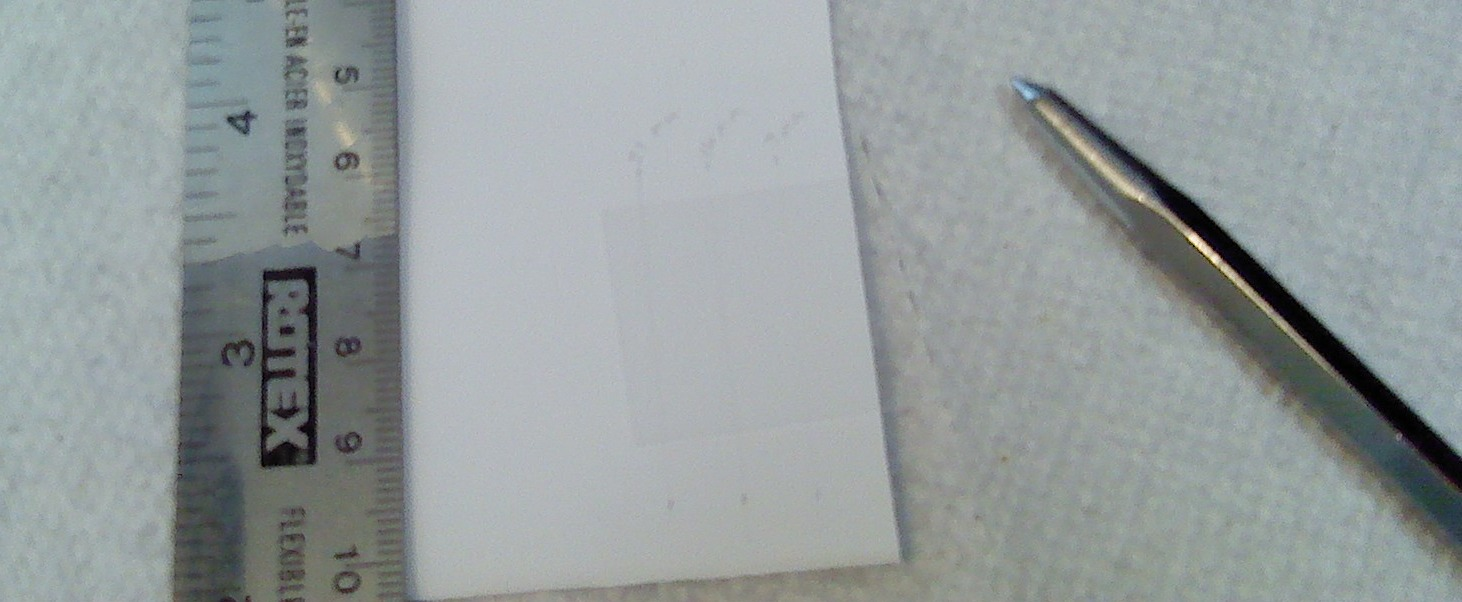
\includegraphics[height=2in]{pics-c920/13-scribingslides.jpg}

The filter plate is 7mm by 7mm by 0.31mm. It must be replaced by one or more
pieces of glass with a total thickness of 0.35mm or more for the camera to
focus properly. This corresponds to the thickness of two \#2 microscope cover
slips (also called ``cover glasses'').

To cut these cover slips, draw guide lines on to a sheet of paper, line
up the edge of the cover slip with one guide line, place a straightedge
over the other guide line, and scribe the glass several times using a
carbide-tipped scribing tool. Carefully snap the cover slip along this line
(holding it with the scribed side facing away from you, and then bending it
so that it bows outwards in that direction).

\textbf{Take extreme care to clean up flakes and slivers of glass.} These
will be produced, and are incredibly sharp (their edges are as thin as a
single atom).

Cut the cover slip sections slightly smaller than 7mm by 7mm; there is no way
to trim them after they are cut.

\section{Wash Cover Slip Plates}

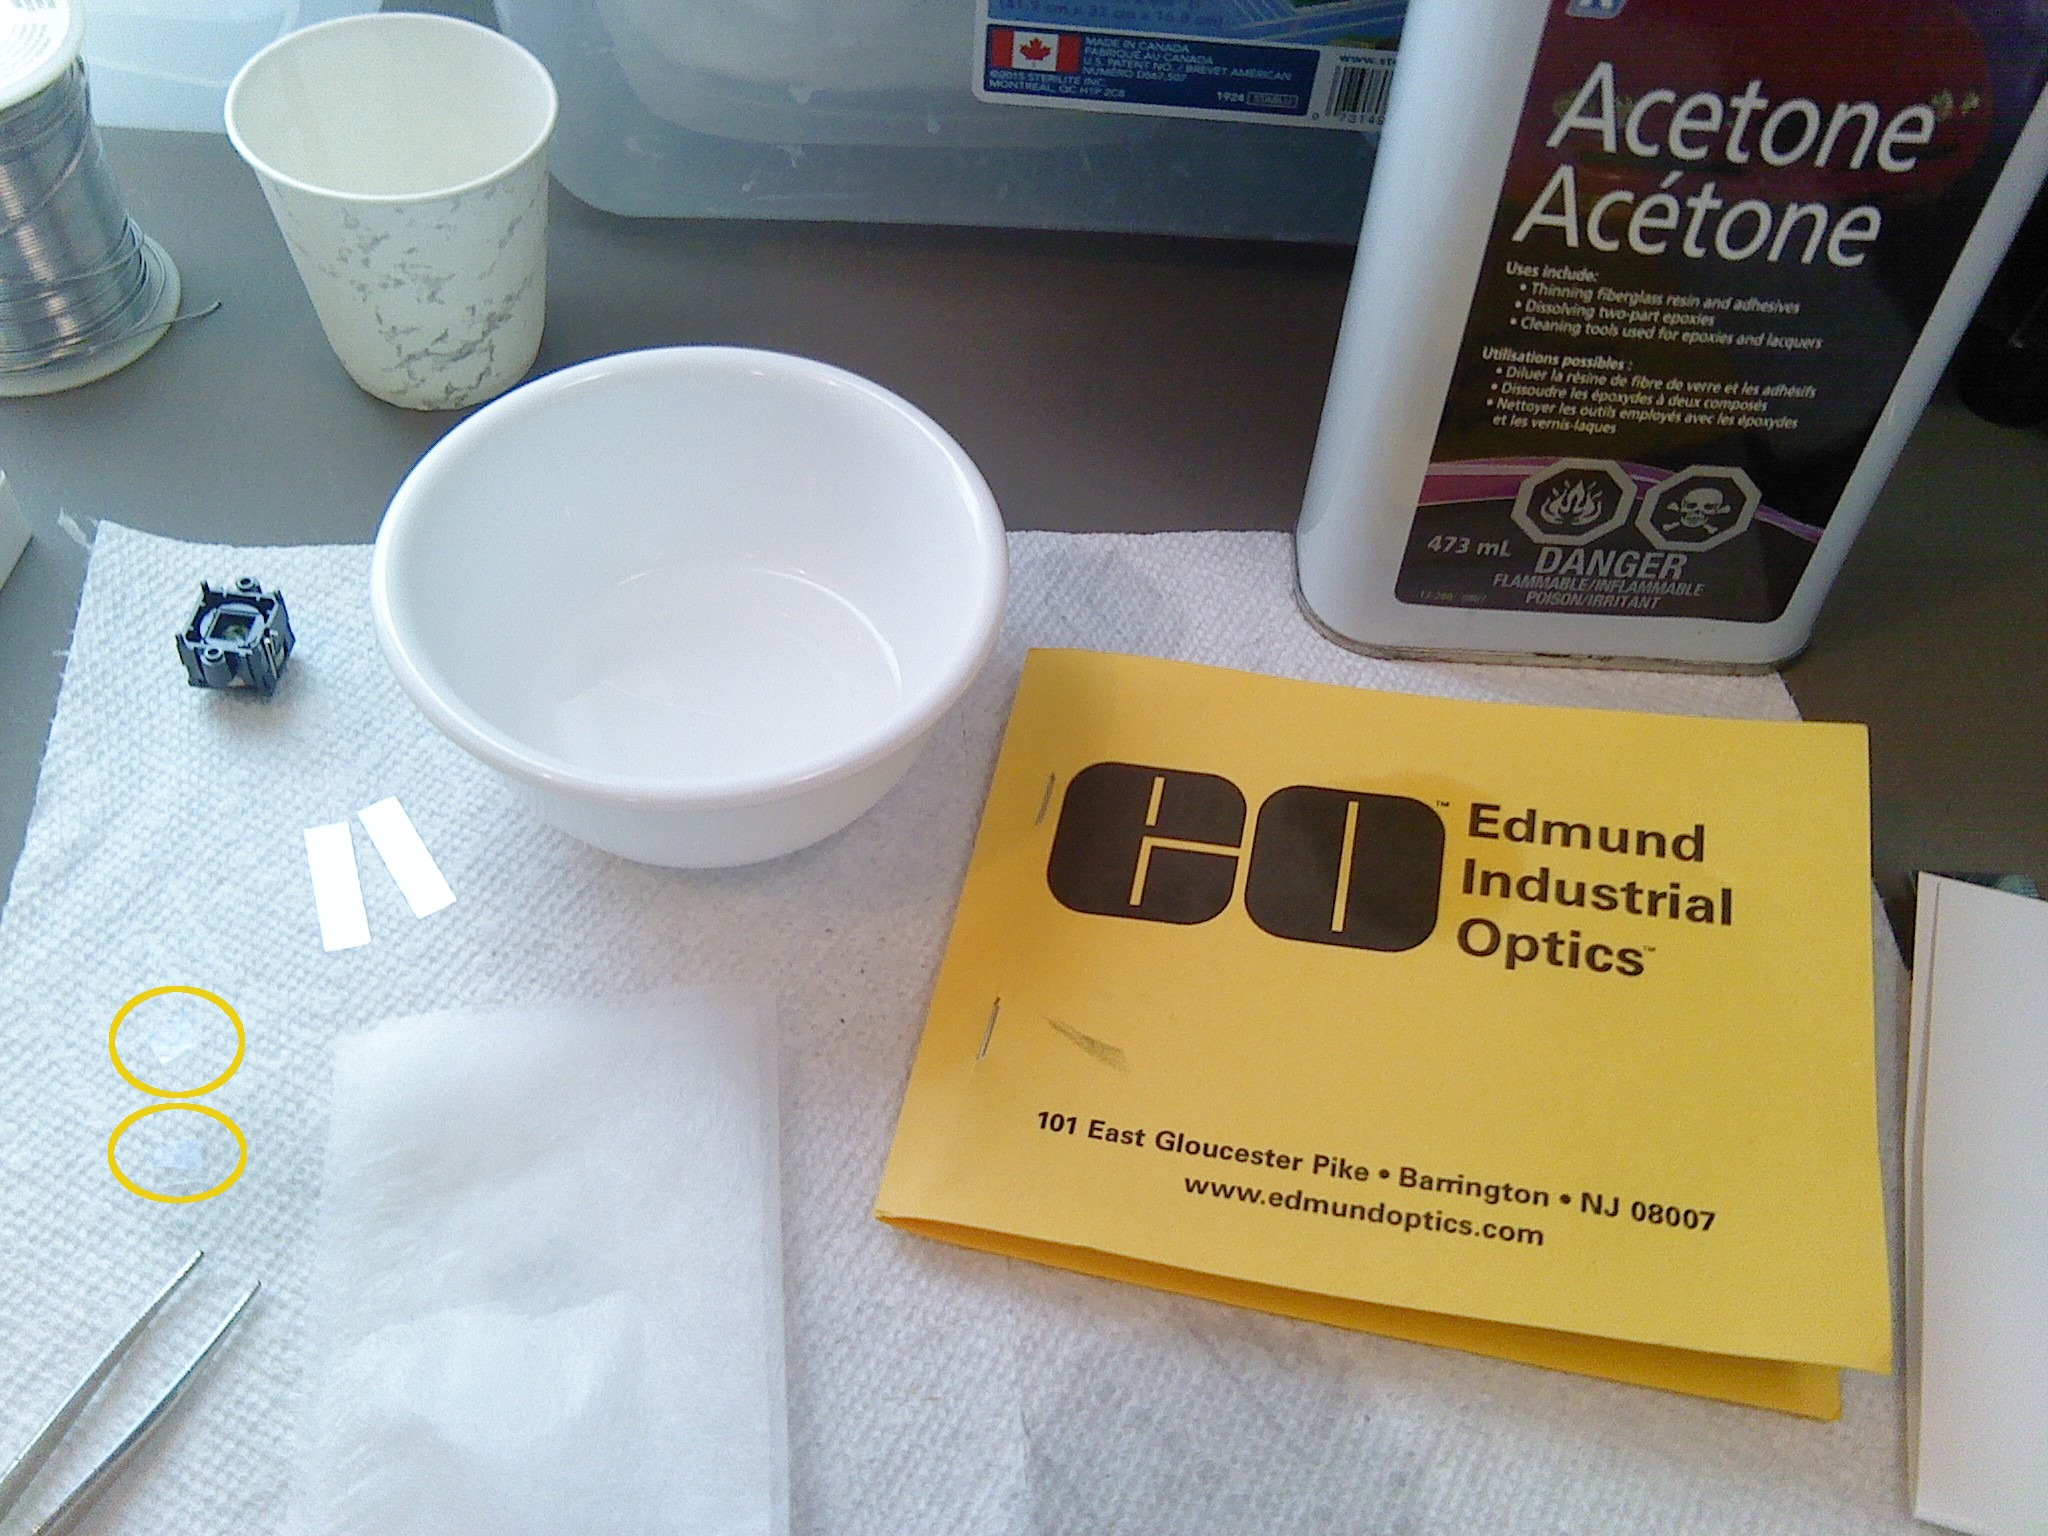
\includegraphics[height=3in]{pics-c920/14-washingslides.jpg}

The cover slip plates must be absolutely free of dust and of oils before
being bonded to the optics assembly. To ensure this, pour acetone into a
small glass or ceramic dish, grasp the edges of a plate with tweezers,
submerge the plate in acetone, and agitate it for a few seconds. Place the
plate onto a dry piece of lens tissue, fold the paper over, and wipe the
plate to remove droplets of acetone and remaining dust. Set clean plates
aside on another piece of lens tissue.

Take care to grasp the plates by the edges, with tweezers. Grasping the
faces will scrape the surfaces of the plates. Squeezing too hard at the
edges will shatter the plates. Grasping faces with fingers will deposit
grease on the plates, and grasping edges with fingers will result in
injury, as snapped edges have atom-thin sharp cusps.

\section{Glue Cover Slip Plates into Optics Assembly}

\includegraphics[height=3in]{pics-c920/15-superglue.jpg}

Carefully stack two cover slip plates into the frame that was occupied by
the IR filter. Carefully apply a bead of cyanoacrylate glue (``super glue'')
to each corner of the frame, wiping the bead outwards (away from the middle
of the plate) when applying it. Wipe each bead again with a piece of lens
tissue to reduce the bead's height.

Do not bond the edges of the frame; just the corners. There has to be ample
space for cyanoacrylate vapours to escape to avoid frosting the plates or
the optics within the assembly. Use a new piece of lens tissue every time
you wipe a bead of glue, to avoid smearing glue on to the cover slip plates.
Be very gentle when applying or wiping glue, to avoid popping the cover slip
plates out of the frame. Cover slip plates can be re-seated using tweezers
if this occurs.

Allow the glue to dry for at least 5 minutes before mounting the optics
assembly back on to the camera board.

%
% This is the end of the file.
